
\subsection{1.18 Невалентные взаимодействия, строение соединений с различными типами невалентных взаимодействий}
Невалентные взаимодействия - взаимодействия без образования
новых химических валентных связей. Обычно они меньше 10-20
ккал/моль. \\
Невалентные взаимодействия могут привести либо к
отталкиванию (электронных оболочек), либо к притяжению. \\ 
К притяжению относятся (даны по убыванию
энергии): 
\begin{itemize}
	\item ион-дипольное взаимодействие
	\item водородные связи
	\item диполь-дипольное взаимодействие
	\item мультипольмультипольное взаимодействие
	\item силы Лондона
\end{itemize} 
Большой разброс по энергии имеют комплексы с
переносом заряда (КПЗ). Энергии притяжения много меньше энергий
ионных и ковалентных взаимодействий. Водородные связи
рассматриваются отдельно. \\ \\
\textbf{Ион-дипольное взаимодействие:} \\
	Молекулярный диполь - система из двух равных и
	противоположных по знаку зарядов $+q$ и $-q$, разделённых расстоянием
	$r$. Тогда дипольный момент $p=qr$. Так как ионом создаётся
	электрическое поле, диполь ориентируется к этому иону за счёт
	притяжения разноимённых зарядов. \\ \\
	Формула ион-дипольного взаимодействия:
	\[
	E_{\text{ион-дип}} = const \cdot \dfrac{|z| \cdot \vec{p} \cdot \overline{e}^2}{r^2}
	\]
	где: $const < 0$ (притяжение с выигрышем по инергии), $z$ - величина заряда иона, $\overline{e}$ - заряд электрона,  $\vec{p}=qr$ - дипольный момент, $r$ - расстояние между ионом и диполем. \\ \\
	Так как дипольный момент является малой величиной, энергия
	ион-дипольного взаимодействия меньше энергии ион-ионного
	взаимодействия. Более того, энергия ион-дипольного
	взаимодействия квадратично убывает с расстоянием, а ионионного - обратно пропорционально:
	\[
	E_{\text{ион-ион}} = const \cdot \dfrac{z^+ \cdot z^- \cdot \overline{e}^2 }{r^2}
	\]
	Такое взаимодействие проявляется при сольватации, когда идёт
	взаимодействие иона с полярной молекулой растворителя. При
	растворении наблюдается очень много таких взаимодействий,
	поэтому энергия сольватации может превысить высокую энергию
	кристаллической решетки, и соединения растворится.  \\ \\
	При этом становится очень важна среда, в которой осуществляется
	то или иное превращение. \\ \\
	\textbf{Диполь-дипольное взаимодействие:} \\
	Крайние случаи взаимодействия диполей:
	
\begin{wrapfigure}{r}{0.15\textwidth}
	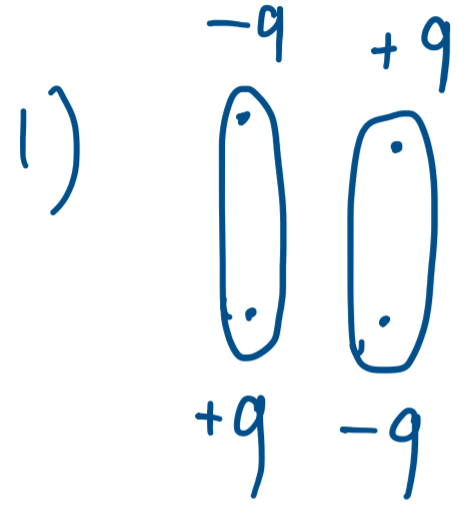
\includegraphics[width=0.15\textwidth]{rr}
\end{wrapfigure}
1) Заряды компенсируются, суммарный дипольный момент равен нулю. 
\\\\\\\\\ \\

\begin{wrapfigure}{l}{0.15\textwidth}
	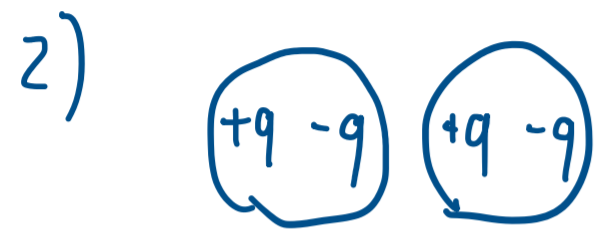
\includegraphics[width=0.15\textwidth]{rr2}
\end{wrapfigure}
2) Расстояние между некомпенсированными зарядами увеличится, суммарный дипольный момент увеличится. \\ \\ 
Энергии обоих вариантов будут одинаковы, если диаметры эллипса
(в условном изображении диполя) относятся, как 1.12:1
\begin{figure} [H]
	\centering {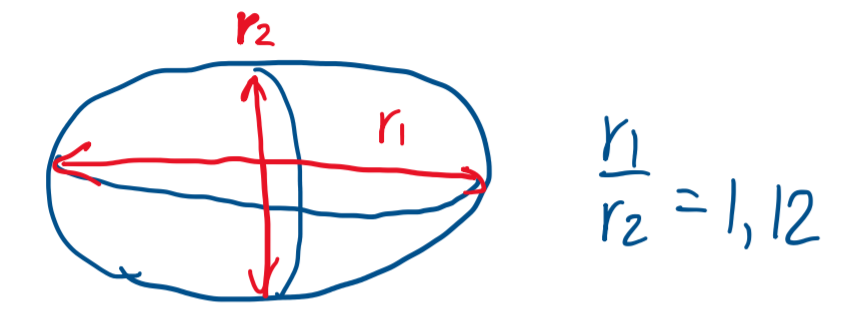
\includegraphics[scale=0.5]{rr3}}
\end{figure}
	\[
	E_{\text{дип-дип}} = const \cdot \dfrac{\vec{p_1}	 \cdot \vec{p_2} }{r^3}
	\]
	Энергия диполь-дипольного взаимодействия убывает с
	расстоянием ещё быстрее, чем энергия ион-дипольного
	вазимодействия. Энергия диполь-дипольного вазимодействия
	невелика, лежит в диапазоне 2.5-5 кДж/моль. \\ \\
	Диполь-дипольные взаимодействия хорошо проявляются при
	низких температурах, при температурах порядка комнатной и выше
	ими можно пренебречь из-за беспорядочного движения молекул. \\ \\ 
	Такое взаимодействие проявляется в таких полярных жидкостях,
	как вода и фтороводород. \\ \\ 
\textbf{Дисперсионное взаимодействие:} \\
Силы Лондона (дисперсионные взаимодействия) - самые слабые.
Их также не очень корректно называют Ван-дер-ваальсовыми
силами (так как зачастую под ним подразумевают и дипольдипольные взаимодействия, и другие). \\ \\
За счёт этого взаимодействия в жидком или твердом состоянии
удерживаются неполярные молекулы (водород, азот, кислород и
т.д.). 
	\[
	E_{\text{дисп}} = const \cdot \dfrac{2 \cdot \vec{p_1}	 \cdot \vec{p_2} }{r^6}
	\]	
\begin{figure} [H]
	\centering {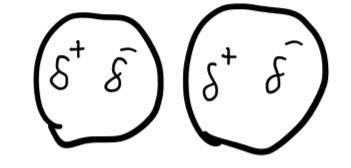
\includegraphics[scale=0.5]{rr4}}
\end{figure}
где $\vec{p_1}, \vec{p_2}$ - мгновенные согласованные диполи. \\
Так как дипольные моменты маленькие, а в знаменателе - шестая
степень, то ничтожные изменения расстояний приводят к
разрушению этих взаимодействий. \\ \\
Фрагмент кристаллической структуры твёрдого хлора:
\begin{figure} [H]
	\centering {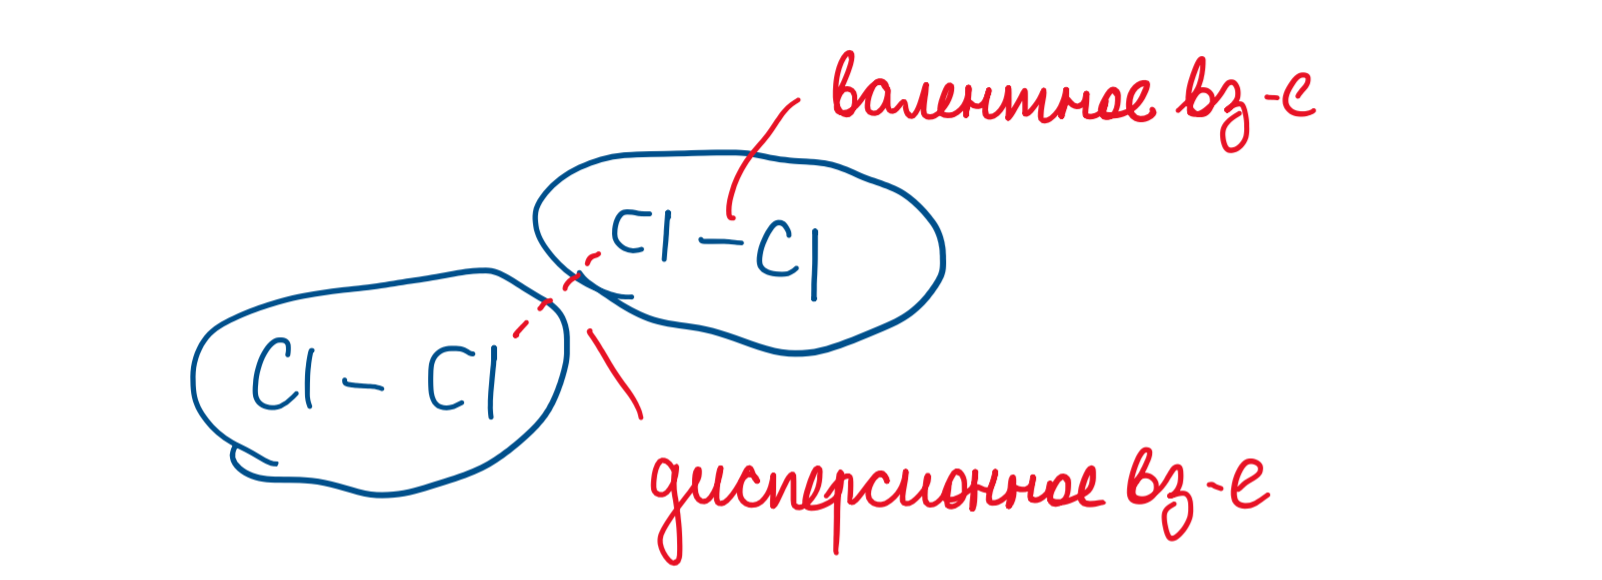
\includegraphics[scale=0.5]{rr5}}
\end{figure}
Величина дисперсионного взаимодействия тут примерно в 10 раз
меньше величины валентного взаимодействия атомов хлора, но всё
равно величина довольно значимая, пренебрегать не стоит. \\ \\
Но, например, для $Li_2$ формула выше неприменима: константа
получится очень большая; при конденсации будут не молекулы, а
кристаллическая решётка. \\ \\
Из расстояния между молекулами в молекулярных кристаллах
вычисляют Ван-дер-ваальсовы радиусы. \\ \\
\textbf{Отталкивание молекул:} \\
При определенном расстоянии между молекулами очень резко
увеличивается, то есть, начинается отталкивание - молекулы
просто не могут подойти ближе. Два атома практически
невозможно вдавить друг в друга. \\ \\
Зависимость энергии взаимодействия молекул от расстояния:
\begin{figure} [H]
	\centering {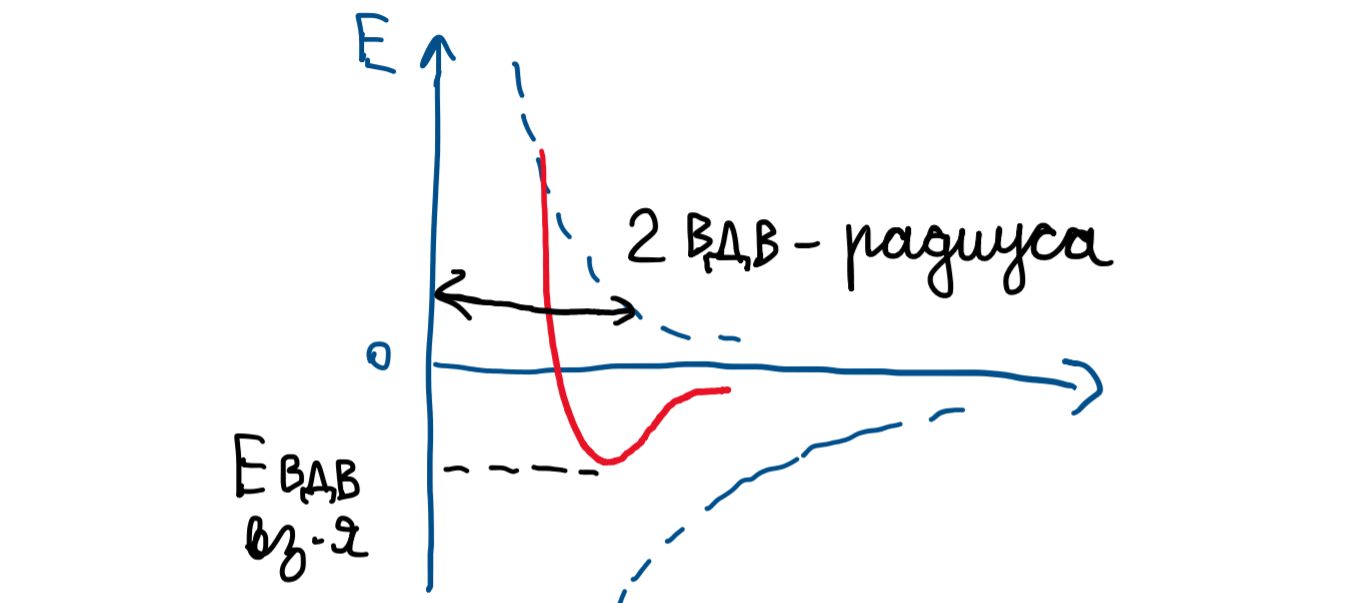
\includegraphics[scale=0.5]{rr6}}
\end{figure}
Заметим, что для атомов водорода в молекуле воды расстояние
между ними значительно меньше, чем два их Ван-дер-ваальсовых
радиуса. То есть, валентные оболочки атомов водорода «вдавлены»
друг в друга. \\ \\
Есть примеры и у углеводородов: расстояния между первым и
третьим атомом в бензоле и противоположными атомами в
циклобутане меньше их двух Ван-дер-ваальсовых радиусов.
\begin{figure} [H]
	\centering {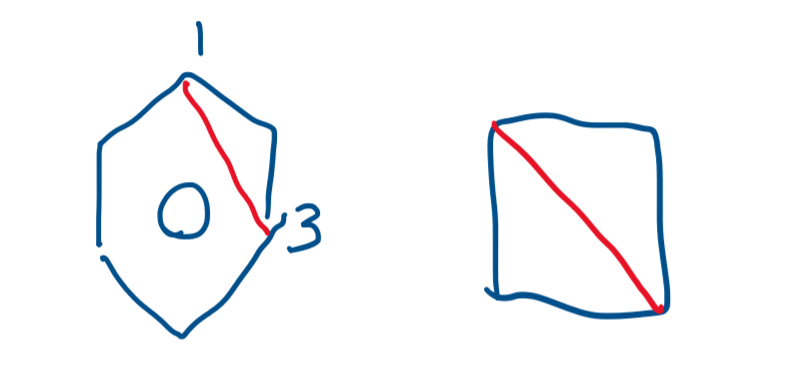
\includegraphics[scale=0.5]{rr7}}
\end{figure}
Энергия отталкивания задаётся выражением:
\[
E_{\text{отталкивания}} = K \cdot r^{-n}, \quad K > 0, n = 5 - 12 \text{ (чаще всего 12)}
\]
Большой показатель степени в знаменателе говорит о том, что при
столкновении молекулы встречают практически твёрдую стенку. \\ \\
\textbf{Комплексы с переносом заряда:} \\
Это можно рассмотреть, как самое слабое донорно-акцепторное
взаимодействие. Эти комплексы очень слабы. Они имеют
небольшой энергетический зазор между связывающей и
разрыхляющей МО (их энергии очень слабо отличаются от
орбитали донора и орбитали акцептора => выигрыш ничтожный),
поэтому спектр поглощения такого комплекса лежит в видимой
области спектра. \\ \\
Посмотрим на реакцию:
\begin{figure} [H]
	\centering {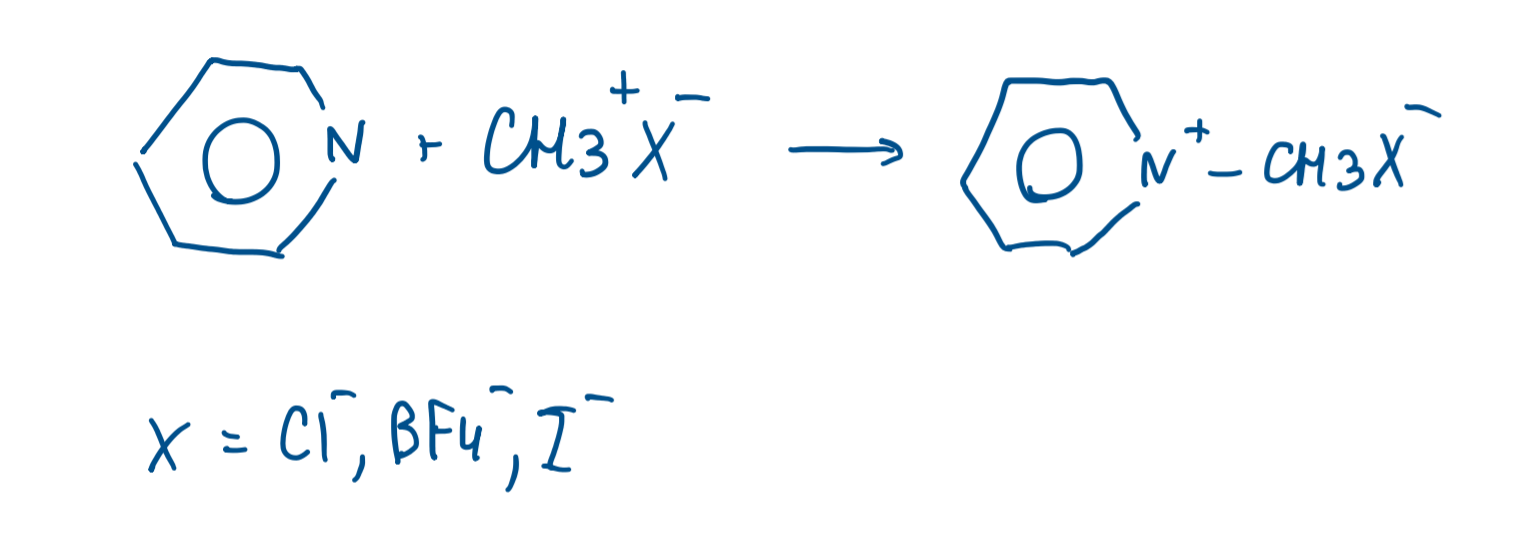
\includegraphics[scale=0.5]{rr8}}
\end{figure}
Все соли, кроме $X=I^-$, бесцветны. Соль с иодидом окрашена, потому
что возникает КПЗ, где анион иода выступает донором, а
акцептором - $\pi$ орбиталь $PyCH_3^+$. \\ \\
Другие примеры КПЗ: диоксан дибромид, $I_3^-$, иод в спирте и в
бензоле.

